\documentclass[11pt,a4paper]{article}
\usepackage[top=1.00in, bottom=1.0in, left=1.1in, right=1.1in]{geometry}
\usepackage{graphicx}
\usepackage{hyperref}
\usepackage[style=authoryear, backend=biber, natbib = true, style=numeric-comp, sortcites, hyperref, sorting=none, giveninits=true, doi=false,isbn=false,url=false,eprint=false, date=year, maxbibnames = 2]{biblatex}
\AtEveryBibitem{\clearfield{pages}}
\AtEveryBibitem{\clearlist{language}}
\AtEveryBibitem{%
  \clearfield{volume}%
  \clearfield{number}}
\AtEveryBibitem{\clearfield{title}}
\renewbibmacro{in:}{}
\usepackage[export]{adjustbox}


\addbibresource{synchrony.bib} 

\begin{document}

\pagenumbering{gobble}

\noindent 
\includegraphics[width=0.5\textwidth, right]{forestry_letterhead.png}

\noindent Dear Dr. X,

\vspace{0.25cm}

\noindent Please consider our paper, entitled ``Solstice optimizes thermal growing season'' for publication as a Brief Communication in \emph{Nature Plants}. 

\vspace{0.25cm}

\noindent Understanding how plants cope with fluctuating climatic conditions has become increasingly important with climate change, across research fields from physiology, ecology, and climatology. Warming has shifted major plant events---leafout, flowering---earlier \supercite{Menzel2006, Fu2019} with potential impacts on growth and, in turn, ecosystem functioning, including carbon storage \supercite{Keenan2014}. These shifts are generally proximately controlled by environmental cues, such as temperature and photoperiod, that plants use to adjust their timing in response to environment variability.

\vspace{0.25cm}

\noindent Summer solstice has recently been proposed as a universal trigger for key physiological processes \supercite{Zohner2023, Journe2024}, with the potential to redefine how we predict plant responses to climate change. This could also reveal a new fundamental mechanism for how plants sense photoperiod. Whether plants rely on solstice, however, is highly debated and has highlighted that we have a limited fundamental understanding of the underlying drivers on the timing of plant transitions. 

\vspace{0.25cm}

\noindent Building on these recent findings, we propose a novel perspective by examining the thermal energy trade-offs that may drive plant phenological transitions. Based on a simple yet powerful approach, we integrate both environmental predictability (plants ability to anticipate environmental conditions) and growth potential (how much more plants can invest in growth) to determine the optimal timing for transitions. Averaging across all of Europe, we found that solstice represents a broad-scale optimum. Yet, our findings also reveal significant variation in the optimal timing across regions. Solstice could just happen to align closely with a thermal cue plants are more likely to track.

\vspace{0.25cm}

\noindent Our results bring a new angle to the solstice debate, with implications for both forecasting plant response to global warming and answering fundamental biological questions. We highlight that future research is still needed to disentangle the role of the solstice as a cue for major phenological transitions. Developing a clearer understanding of the optimal drivers of transitions will be critical to better simulate plant phenology on a global scale as well as to understand the long-term adaptive responses of plant communities more broadly. 

\vspace{0.25cm}

\noindent Both authors contributed to this work and approve this version for submission. The manuscript is 1141 words, with 14 references and 2 figures, and is not under consideration elsewhere. We hope you find it suitable for publication in \emph{Nature Plants}, and look forward to hearing from you. 

\vspace{0.45cm}
\noindent Sincerely, 
\vspace{0.35cm}\\
\hspace*{-0.5cm}
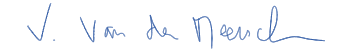
\includegraphics[scale=.65]{sign_long.png} \\
\noindent Victor Van der Meersch, PhD\\
\noindent \emph{Forest \& Conservation Sciences}\\
\noindent \emph{University of British Columbia}

\clearpage

\paragraph{References}
\printbibliography[heading=none]


\newpage

\end{document}


